\documentclass[a4paper,11pt]{article}
\author{ 杨旭鹏  \  PB17000234}
\date{2019年秋季}
\title{计算物理A 第十六题}

\usepackage{ctex}
\usepackage{amsmath}
\usepackage{amsfonts}
\usepackage{graphicx}
\usepackage{epstopdf}
\usepackage{lastpage}
\usepackage{hyperref}
\usepackage{listings}
\RequirePackage{xcolor}
\usepackage{appendix}
\usepackage{caption2}
\usepackage{subfigure}
\usepackage{float}
\usepackage{verbatim}
\usepackage{fancybox}
\usepackage{geometry}
\geometry{left=3cm,right=3cm,top=2.5cm,bottom=2.5cm}
\makeatletter\def\@captype{table}\makeatother
\usepackage{tikz}
\usetikzlibrary{shapes,arrows}
\tikzstyle{startstop} = [rectangle,rounded corners, minimum width=3cm,minimum height=1cm,text centered, draw=black,fill=red!30]
\tikzstyle{io} = [trapezium, trapezium left angle = 70,trapezium right angle=110,minimum width=3cm,minimum height=1cm,text centered,draw=black,fill=blue!30]
\tikzstyle{process} = [rectangle,minimum width=4cm,minimum height=1cm,text centered, text width=3.5cm, draw=black,fill=orange!30]
\tikzstyle{decision} = [diamond,minimum width=3cm,minimum height=1cm,text centered,draw=black,fill=green!30]
\tikzstyle{arrow} = [thick,->,>=stealth]


\definecolor{dkgreen}{rgb}{0,0.6,0}
\definecolor{gray}{rgb}{0.5,0.5,0.5}
\definecolor{mauve}{rgb}{0.58,0,0.82}

\lstset{
  frame=tb,
  aboveskip=3mm,
  belowskip=3mm,
  showstringspaces=false,
  columns=flexible,
  framerule=1pt,
  rulecolor=\color{gray!35},
  backgroundcolor=\color{gray!5},
  basicstyle={\small\ttfamily},
  numbers=left,
  numberstyle=\tiny\color{gray},
  keywordstyle=\color{blue},
  commentstyle=\color{dkgreen},
  stringstyle=\color{mauve},
  breaklines=true,
  breakatwhitespace=true,
  tabsize=3,            
  }



\begin{document}
\maketitle
\tableofcontents

\section{题目描述}
设体系能量为$H(x,y) = \frac{x^{2}}{2\sigma_{x}^{2}} + \frac{y^{2}}{2\sigma_{y}^{2}}$(以$kT$为单位),采用Metropolis抽样法计算 $\left < x^{2}  \right > , \left < y^{2}  \right > , \left < x^{2} + y^{2}  \right > $,并与解析结果进行比较。抽样时在2维平面上依次标出Markov 链点分布,从而形象地理解Markov链。

\section{理论推导}
设体系满足Boltzman分布,则有:
\begin{equation}
	p(x,y) = \frac{1}{Z} e^{  -H(x,y)/kT }
\end{equation}
其中$Z$为配分函数,即:
\begin{equation}
	Z = \int_{-\infty}^{\infty} \int_{-\infty}^{\infty} e^{ - \left(   \frac{x^{2}}{2\sigma_{x}^{2}} + \frac{y^{2}}{2\sigma_{y}^{2}}  \right) } dx dy = 2\pi \sigma_{x} \sigma_{y}
\end{equation}
则可知有:
\begin{equation}
	p(x,y) = \frac{e^{  -   \left(   \frac{x^{2}}{2\sigma_{x}^{2}} + \frac{y^{2}}{2\sigma_{y}^{2}}  \right)  }}{2\pi \sigma_{x} \sigma_{y}}
\end{equation}

则有:
\begin{equation}
	\left < x^{2}  \right > =  \int_{-\infty}^{\infty} \int_{-\infty}^{\infty}  x^{2} \frac{e^{  -   \left(   \frac{x^{2}}{2\sigma_{x}^{2}} + \frac{y^{2}}{2\sigma_{y}^{2}}  \right)  }}{2\pi \sigma_{x} \sigma_{y}} dx dy = \sigma_{x}^{2}
\end{equation}

\begin{equation}
	\left < y^{2}  \right > =  \int_{-\infty}^{\infty} \int_{-\infty}^{\infty}  y^{2} \frac{e^{  -   \left(   \frac{x^{2}}{2\sigma_{x}^{2}} + \frac{y^{2}}{2\sigma_{y}^{2}}  \right)  }}{2\pi \sigma_{x} \sigma_{y}} dx dy = \sigma_{y}^{2}
\end{equation}

\begin{equation}
	\left < x^{2} + y^{2}  \right > = \sigma_{x}^{2} + \sigma_{y}^{2}
\end{equation}

\section{Metropolis算法}

\begin{tikzpicture}[node distance=2cm]
\node (start) [startstop] {起始点$(x_{0},y_{0})$};
\node (gen1) [process,below of=start] {产生在$(-\Delta,\Delta)$均匀分布的随机数$\delta x,\delta y$};
\node (next2) [process,right of=gen1,xshift = 3cm]{进行下一轮计算 \\ $n+1$};
\node (dE) [process,below of=gen1]{计算能量差 \\ $\Delta E  = E_{n+1}-E_{n}$};
\node (decision1) [decision,below of = dE ,yshift=-0.5cm] {$\Delta E <0$};
\node (next1) [process,left of = decision1,xshift = -2cm]{进行下一轮计算 \\ $n+1$};
\node (gen2) [process,right of =decision1,xshift=2.5cm] {产生在[0,1]间均匀分布的随机数$\xi$};
\node (decision2) [decision,right of =gen2,xshift=2cm] {$\xi < e^{-\Delta E}$};
\node(value2) [process,above of=decision2,yshift = 0.6cm]{$x_{n+1} = x_{n} $ \\ $ y_{n+1} = y_{n} $};
\node (value) [process,below of=decision1,yshift=-0.5cm] {$x_{n+1} = x_{n} + \delta  x$ \\ $ y_{n+1} = y_{n} + \delta y$};
\node (decision3) [decision,below of = value ,yshift=-0.5cm] {$n<N$};
\node (end) [startstop, below of = decision3] {程序结束};


\draw [arrow] (start) -- (gen1);
\draw [arrow] (gen1) -- (dE);
\draw [arrow] (dE) -- (decision1);
\draw [arrow] (decision1) -- node[anchor=south] {no} (gen2);
\draw [arrow] (decision1) -- node[anchor=west] {yes} (value);
\draw [arrow] (gen2) -- (decision2);
\draw [arrow] (decision2) --  node[anchor=west] {no}(value2);
\draw [arrow] (decision2) |-  node[anchor=west] {yes}(value);
\draw [arrow] (value2) |- (next2);
\draw [arrow] (next2) -- (gen1);
\draw [arrow] (value) -- (decision3);
\draw [arrow] (decision3) -- node[anchor=west] {yes} (end);
\draw [arrow] (decision3) -| node[anchor=north] {no} (next1);
\draw [arrow] (next1) |- (gen1);
\end{tikzpicture}

算法流程图如上所示。


\section{程序使用方法}
此程序设计为参数在程序代码中直接赋值形式,每次需在程序源码中进行参数调整,进而编译运行,以简化每次输入的过程(重复运行时不用在此输入)。需要调整的参数包括main函数中的Markov链总链节数$N$,初始链节的坐标,体系能量表达式中的参数$\sigma_{x},\sigma_{y}$,每一步的步长参数$\Delta$,算统计量所需排除的初始链节个数。调整完参数后,编译运行,程序会自动输出Markov链节$(x,y)$坐标至不同文件并在屏幕上打印出统计量的计算结果。


\section{程序结果与讨论}
当设定起始点的坐标为$(10,10), \sigma_{x} = \sigma_{y} = 1$时,得到结果:

\begin{figure}[!htbp]   
\centering     
\subfigure[$\Delta = 0.1$得到的Markov链]{
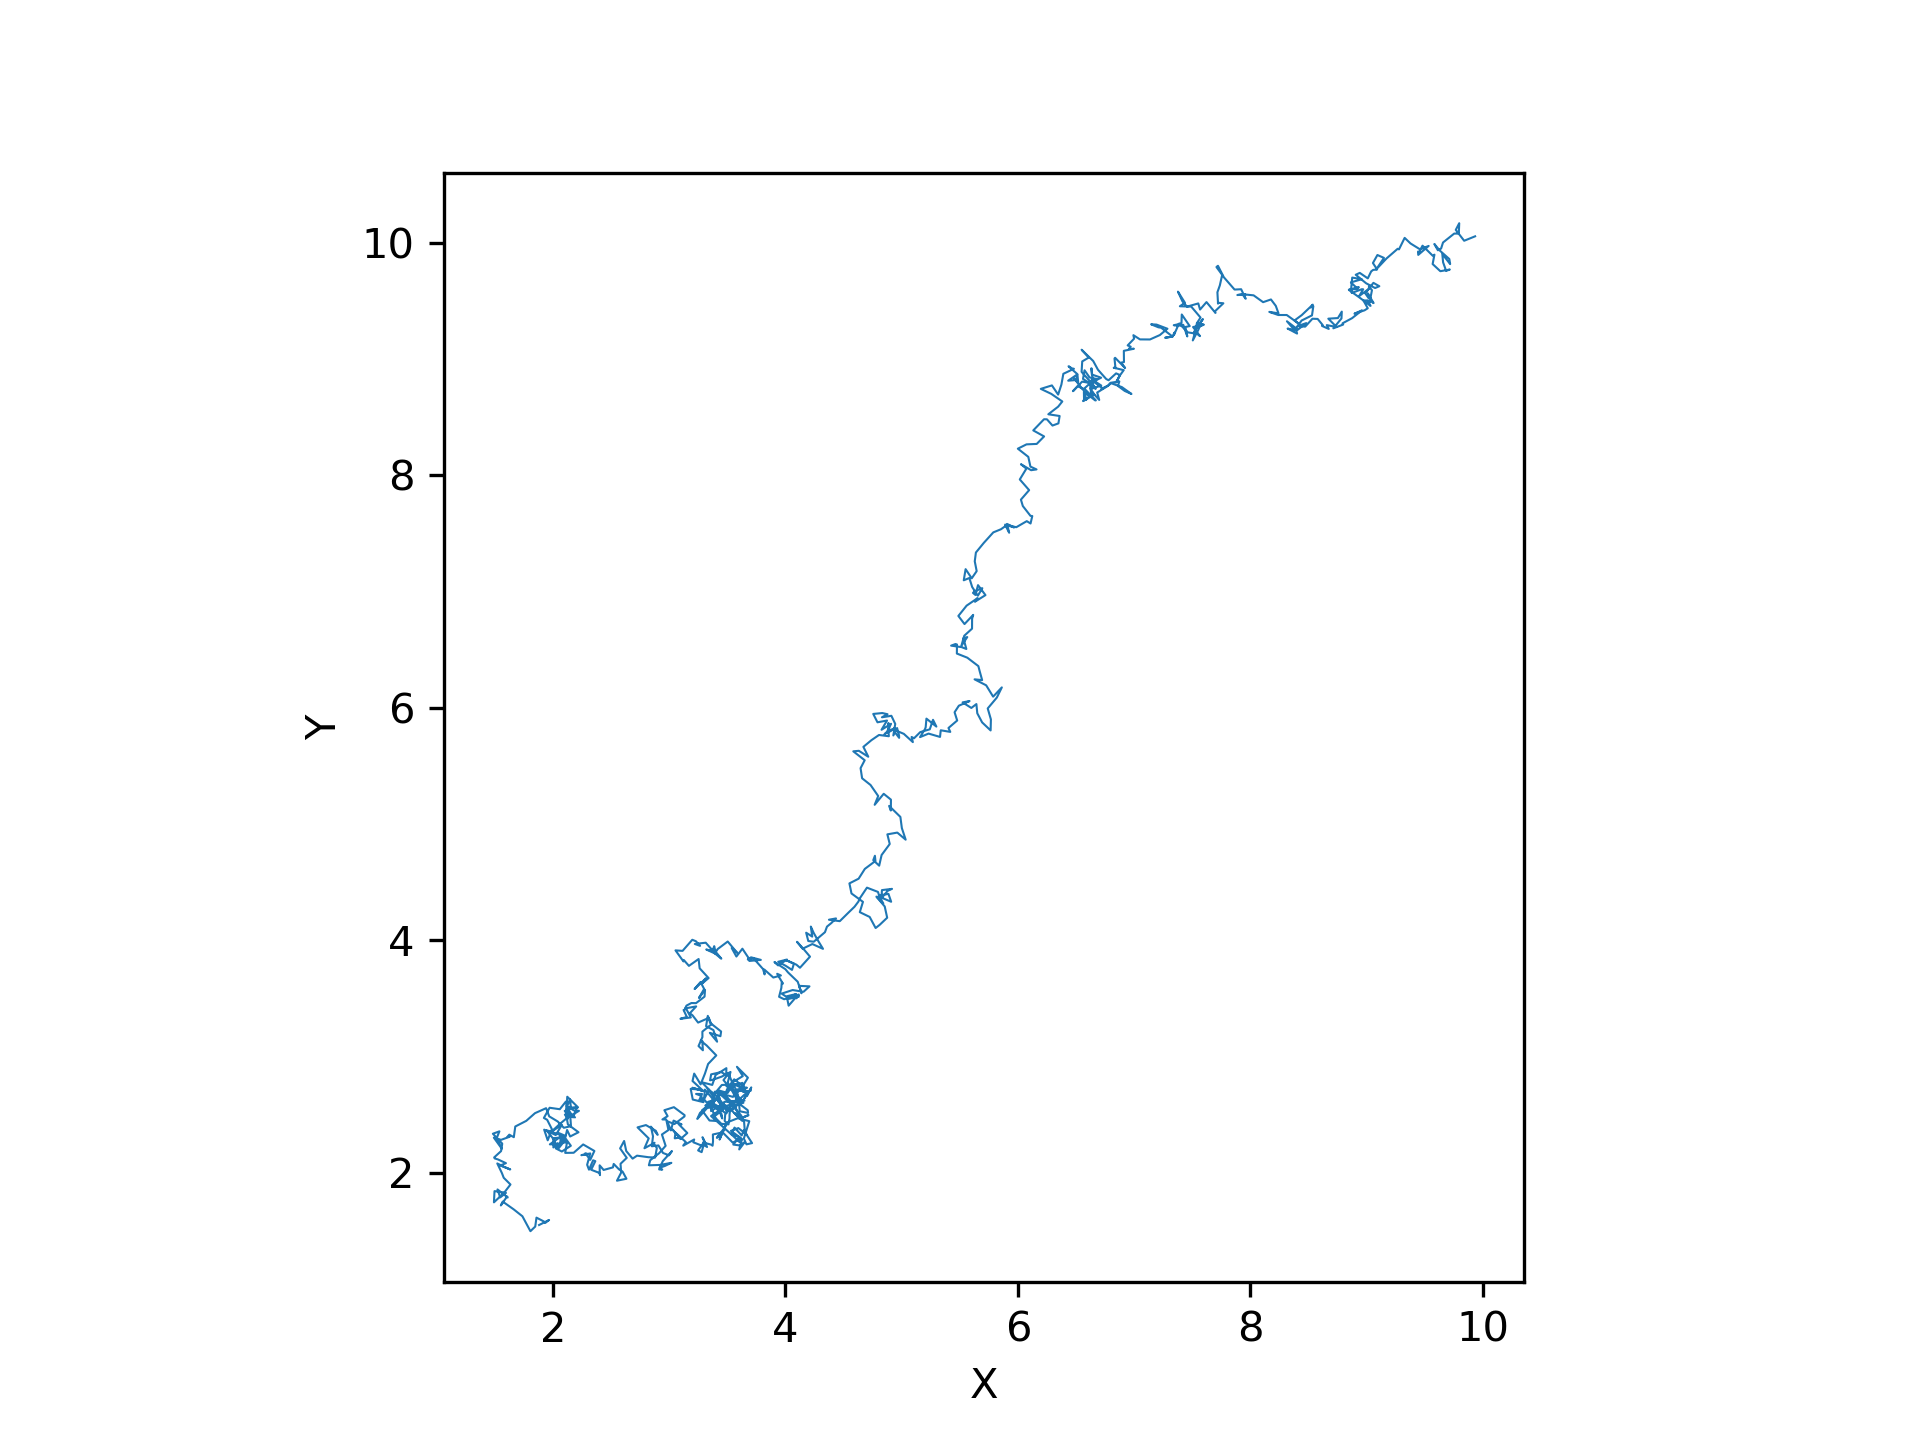
\includegraphics[bb= 0 0 460.8 345.6,width=6cm] {0.1-103-2.png}
}
\subfigure[$\Delta = 0.5$得到的Markov链]{
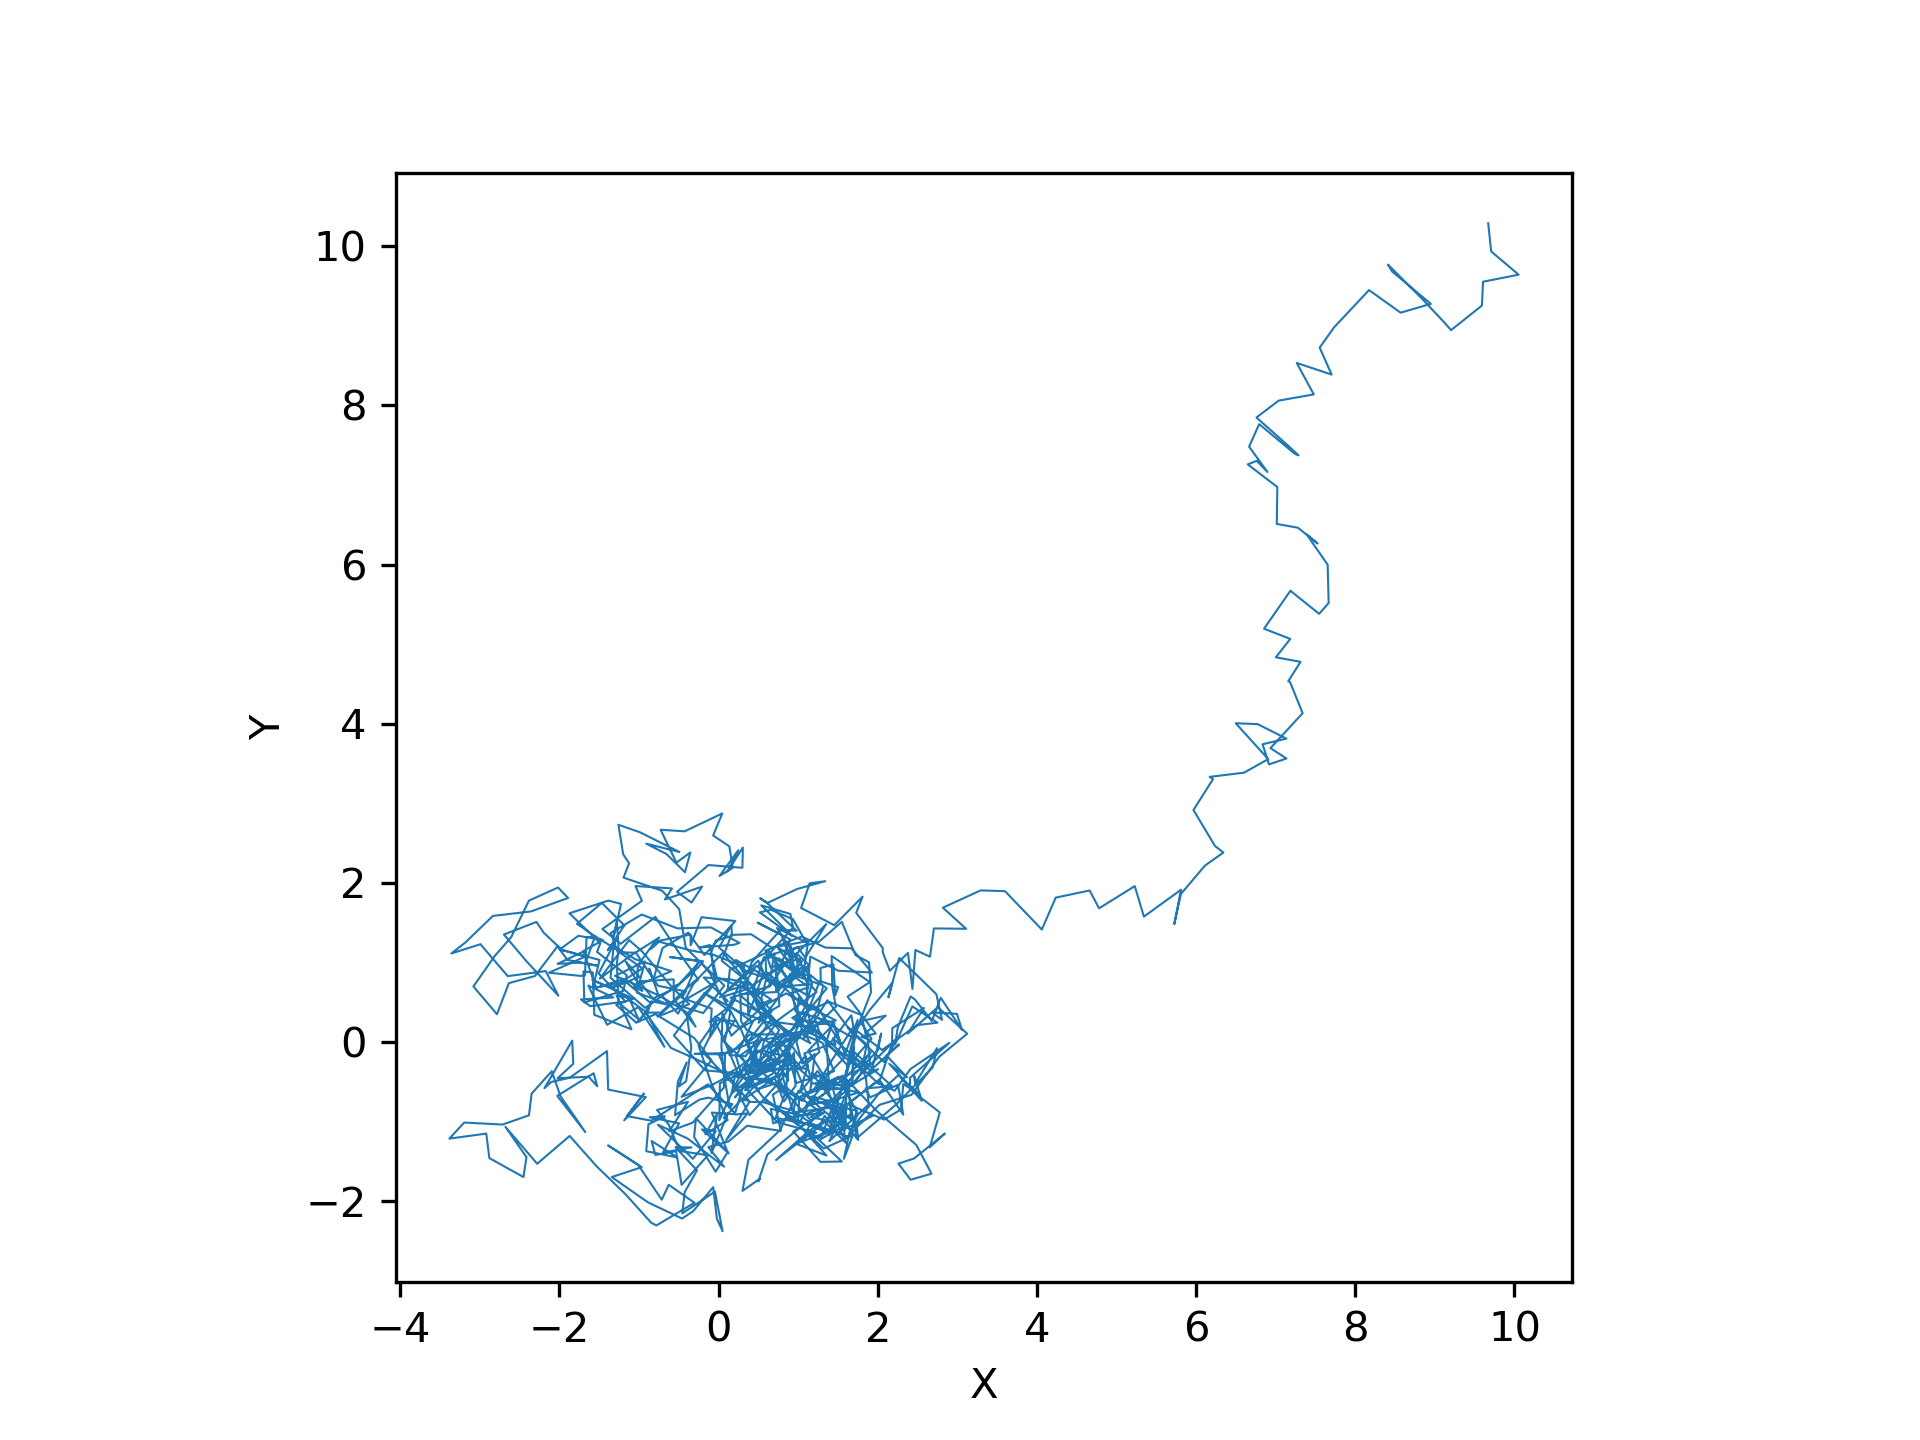
\includegraphics[bb= 0 0 460.8 345.6,width=6cm] {0.5-103-2.png}
}       
\subfigure[$\Delta = 1$得到的Markov链]{
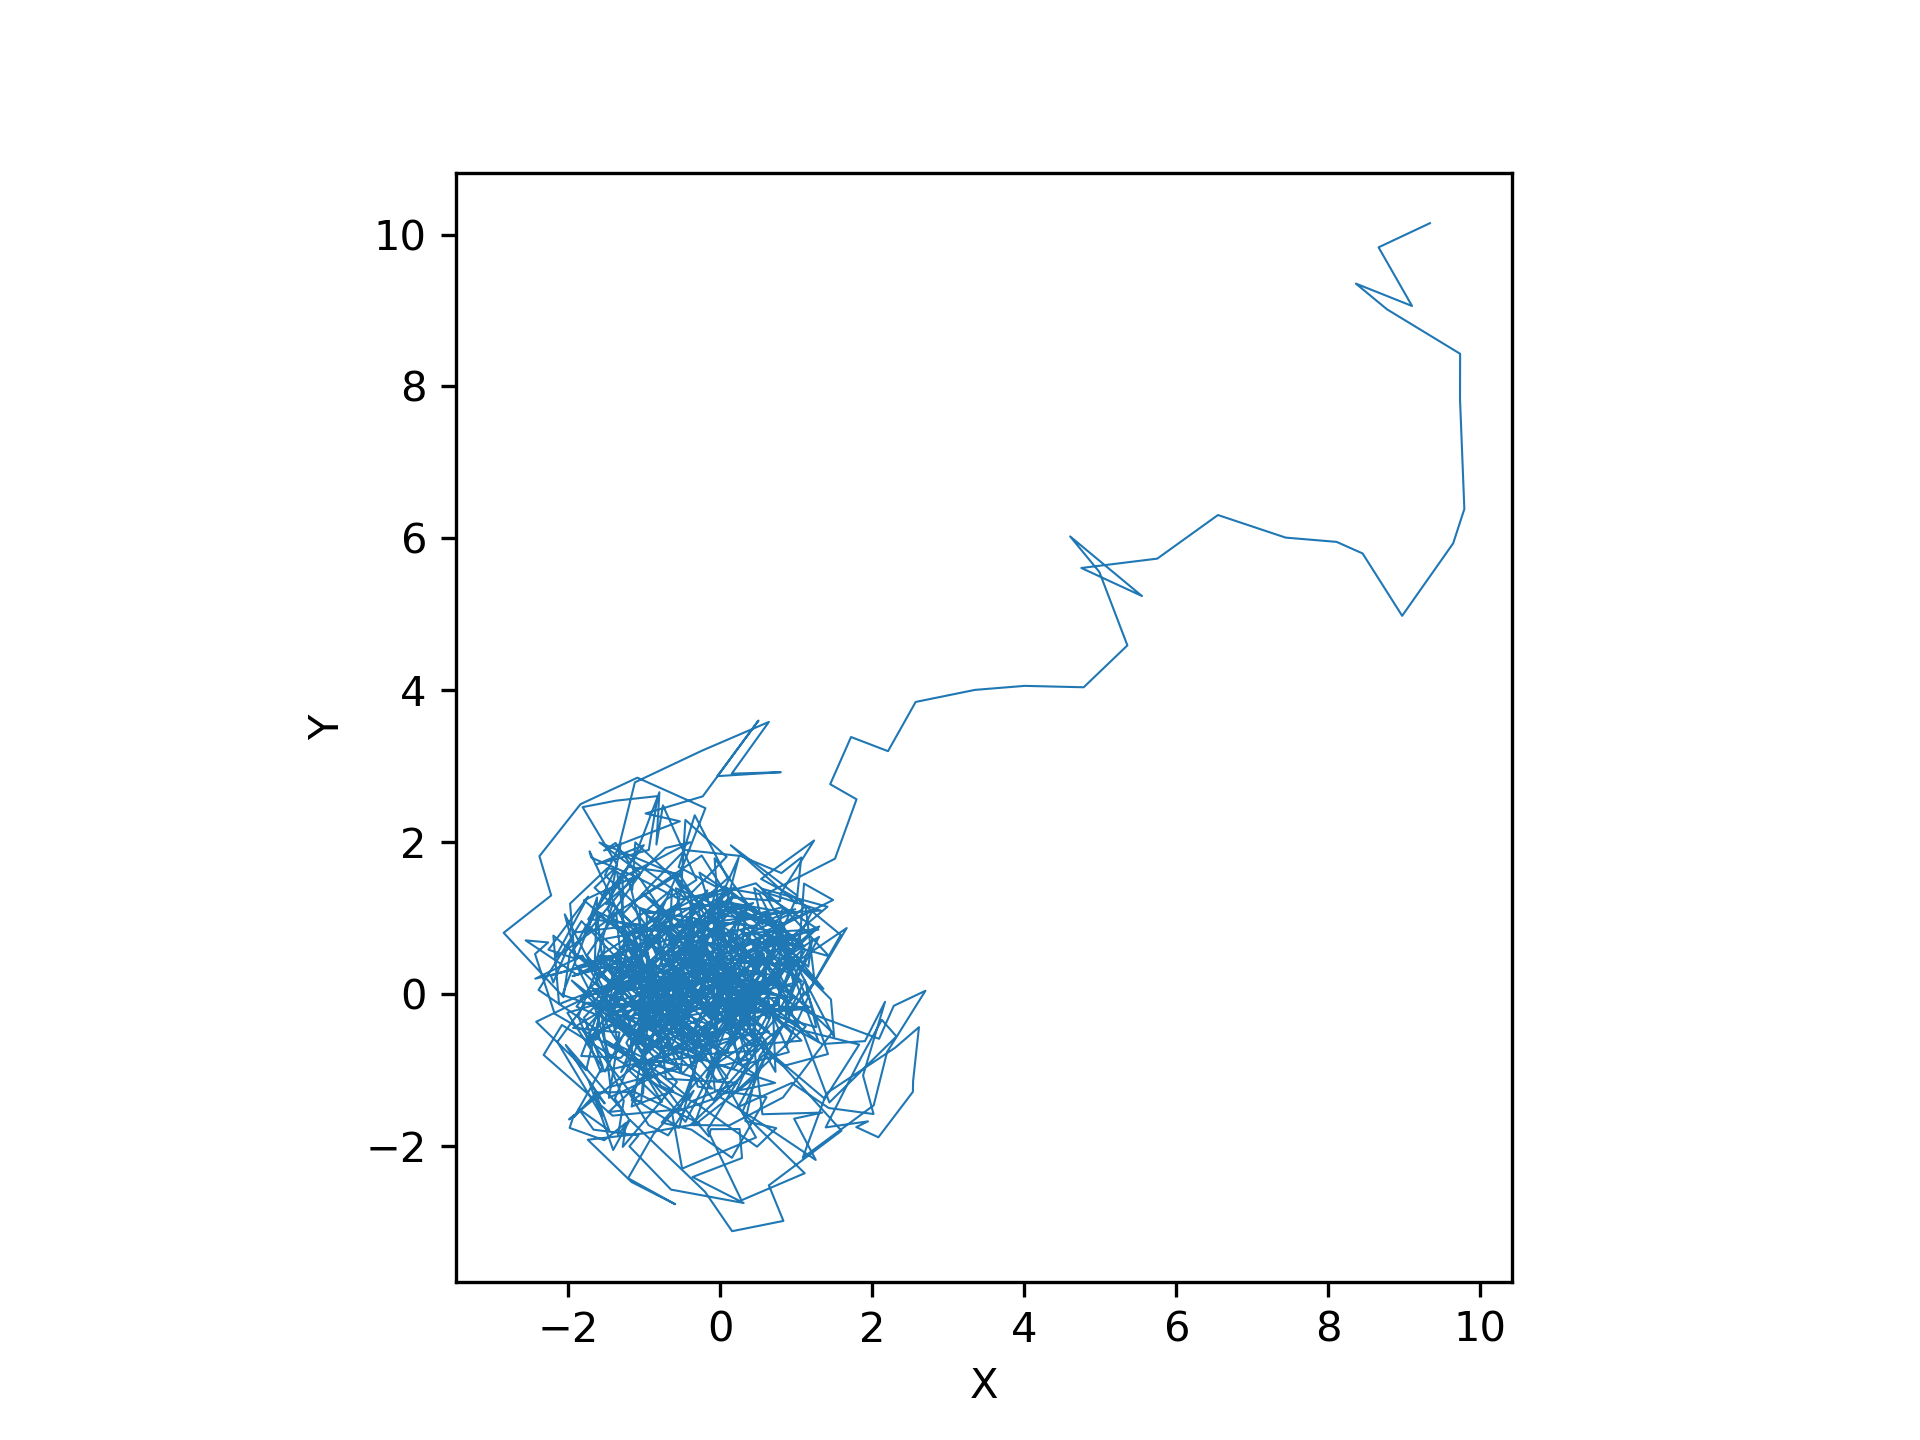
\includegraphics[bb= 0 0 460.8 345.6,width=6cm] {1-103-2.png}
}                
\caption{$ N = 10^{3} $得到的Markov链}      
\end{figure}


\begin{figure}[!htbp]   
\centering     
\subfigure[$\Delta = 0.1$得到的Markov链]{
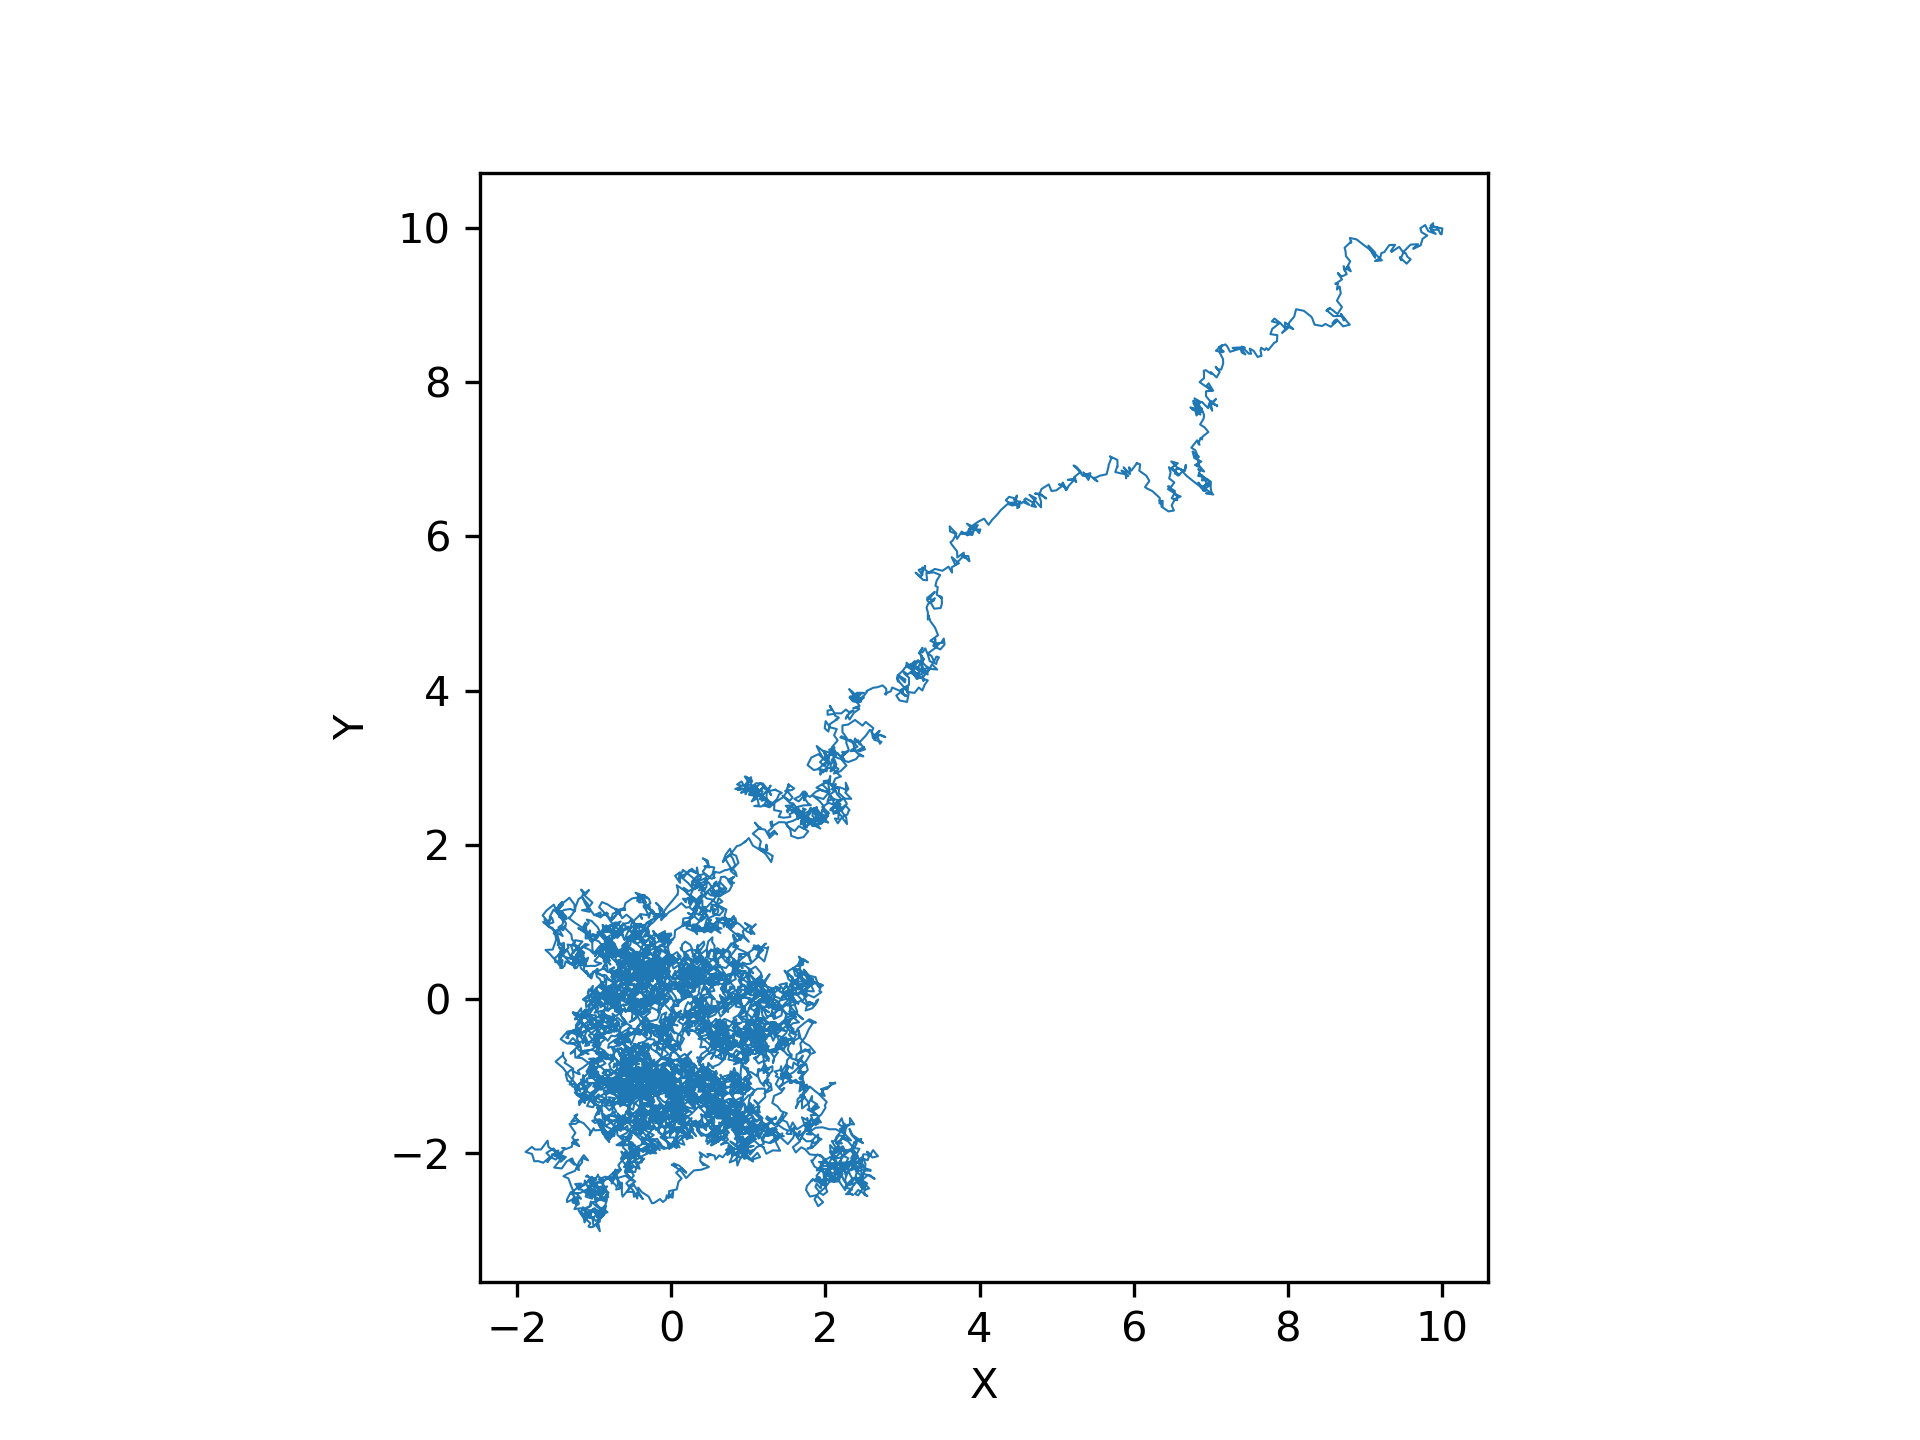
\includegraphics[bb= 0 0 460.8 345.6,width=6cm] {0.1-104-2.png}
}
\subfigure[$\Delta = 0.5$得到的Markov链]{
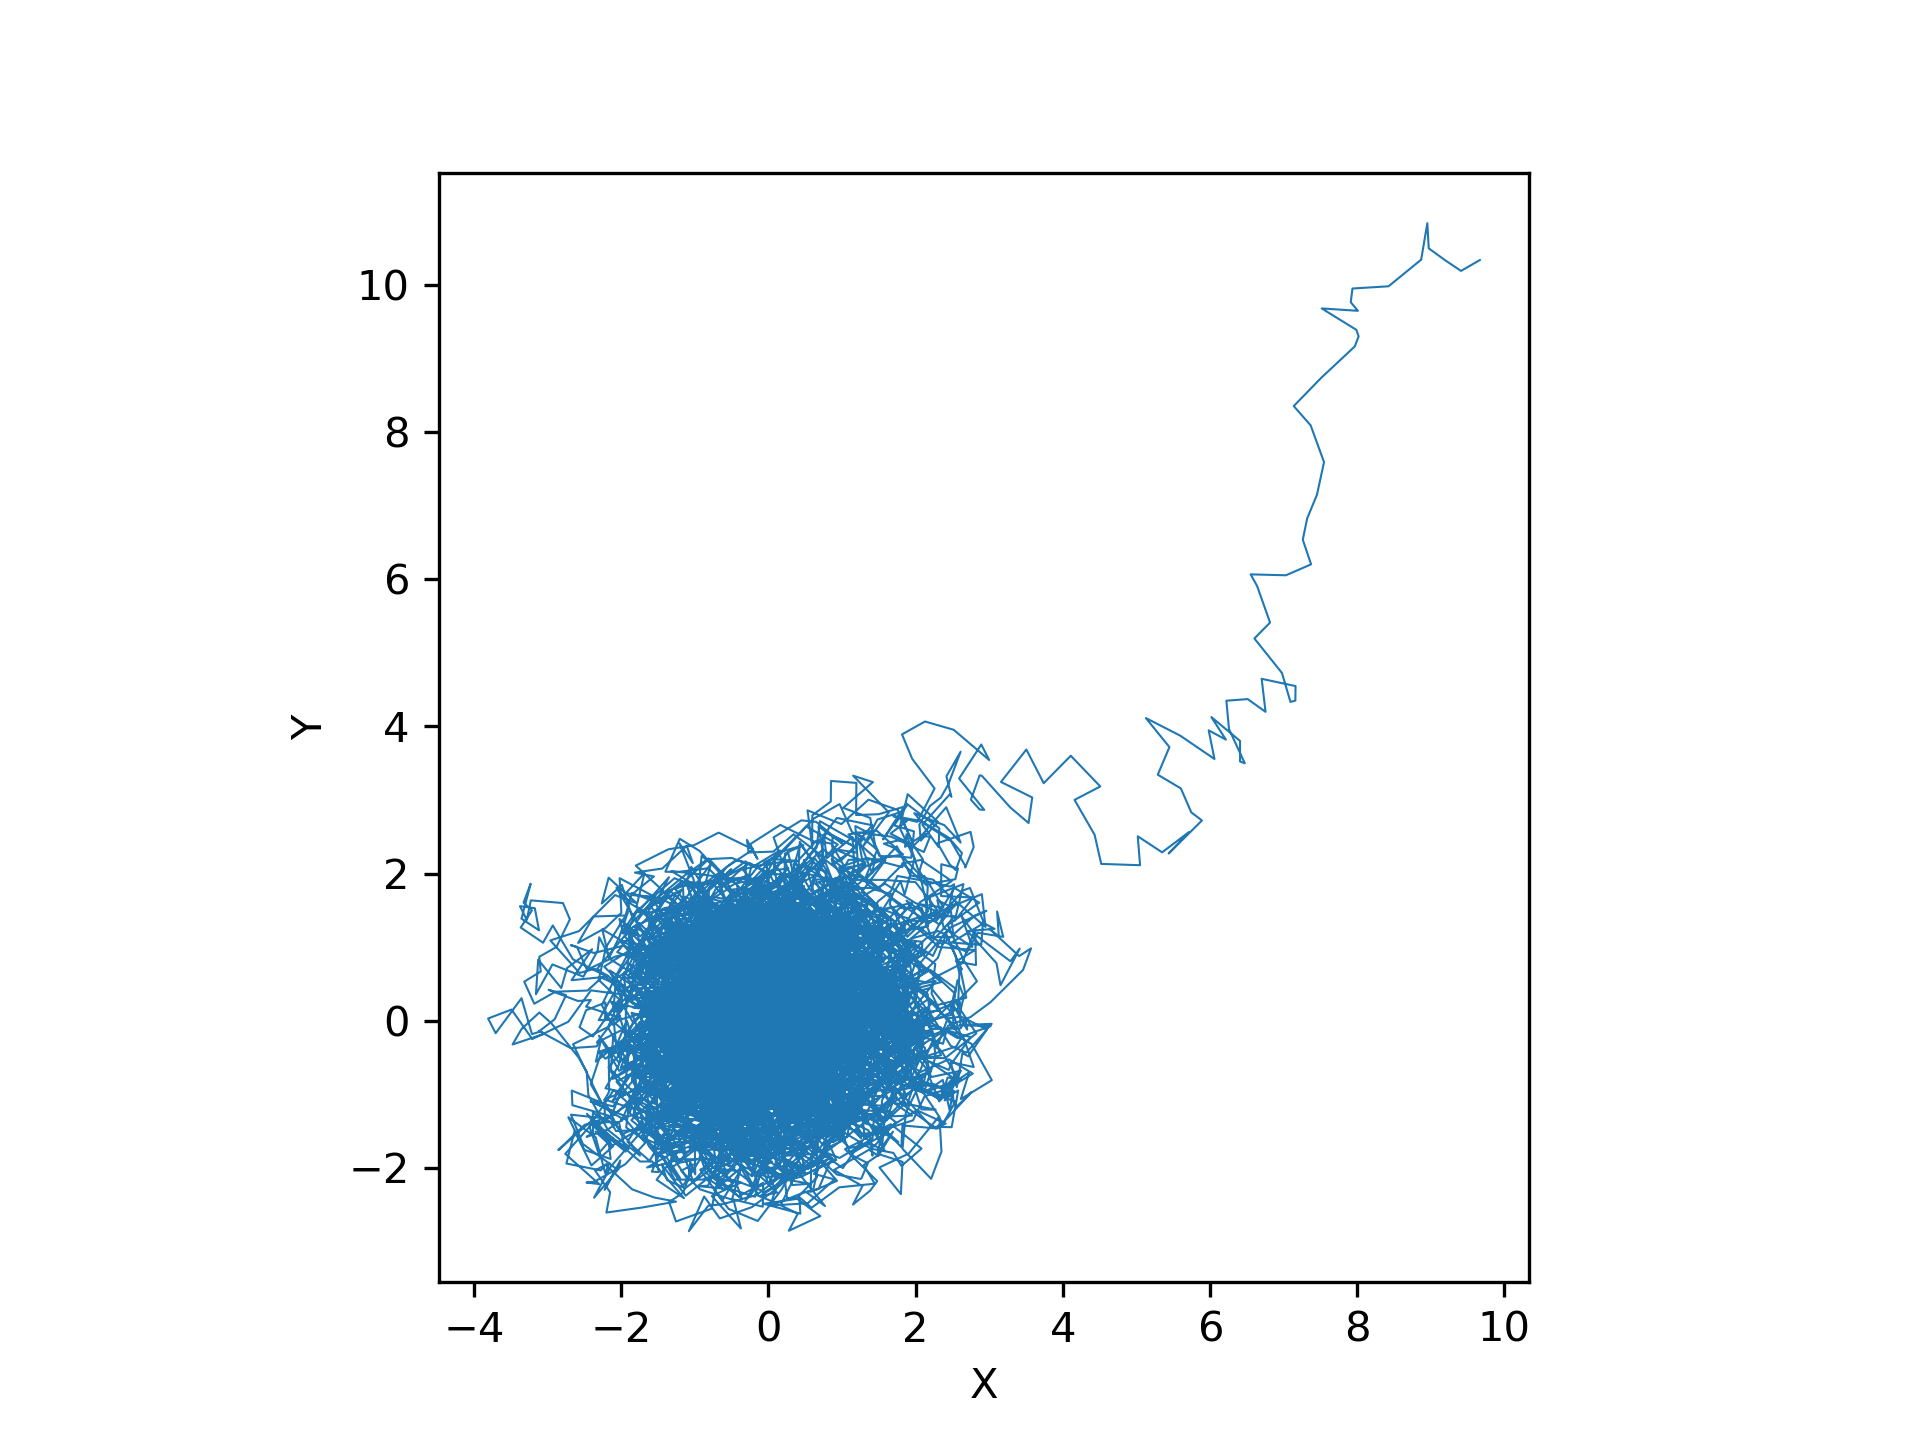
\includegraphics[bb= 0 0 460.8 345.6,width=6cm] {0.5-104-2.png}
}       
\subfigure[$\Delta = 1$得到的Markov链]{
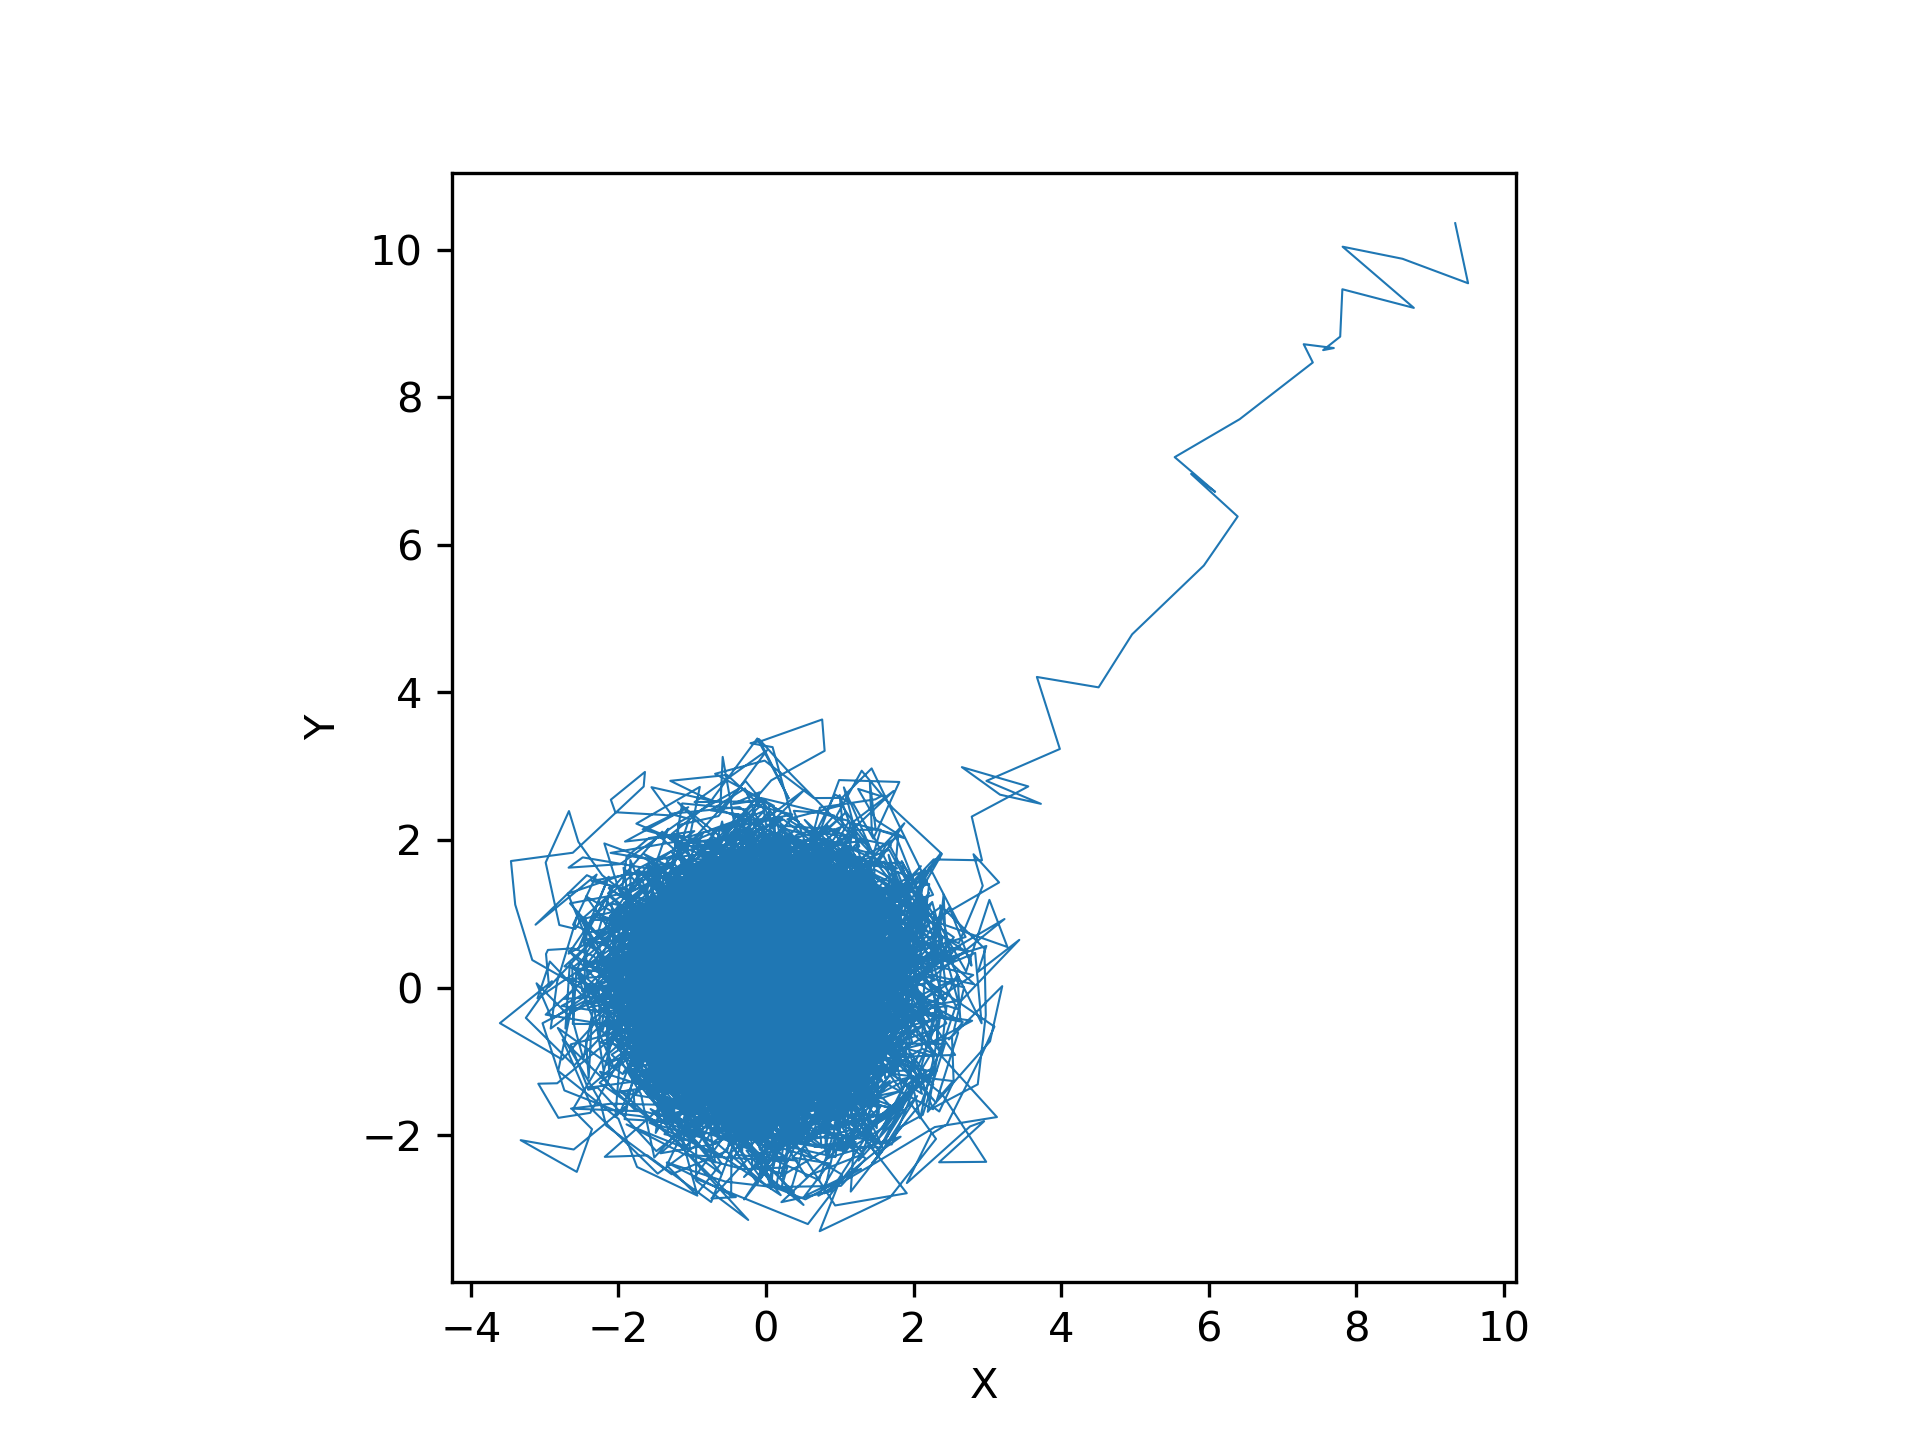
\includegraphics[bb= 0 0 460.8 345.6,width=6cm] {1-104-2.png}
}                
\caption{$ N = 10^{4} $得到的Markov链}      
\end{figure}

\newpage
可以很明显的看出随着步长的增加,Markov链节更加快速的收敛到概率值最大的地方附近,并在相同链节数的情况下,在概率值附近更加均匀。由于最后得到的是抽样得到Markov链节,而不是Markov链本身,故此时可认为步数大一点会使程序抽样效率更高。

为了计算统计量,我们将前$n$个链节数据删除,以排除初始位置对于统计量计算的影响。例如对于$N=10^{6}$的情况,我们删除前$n$个链节有可视化结果:

\begin{figure}[!htbp]
\centering
\subfigure[$\Delta = 0.05,n=5000$得到的Markov链]{
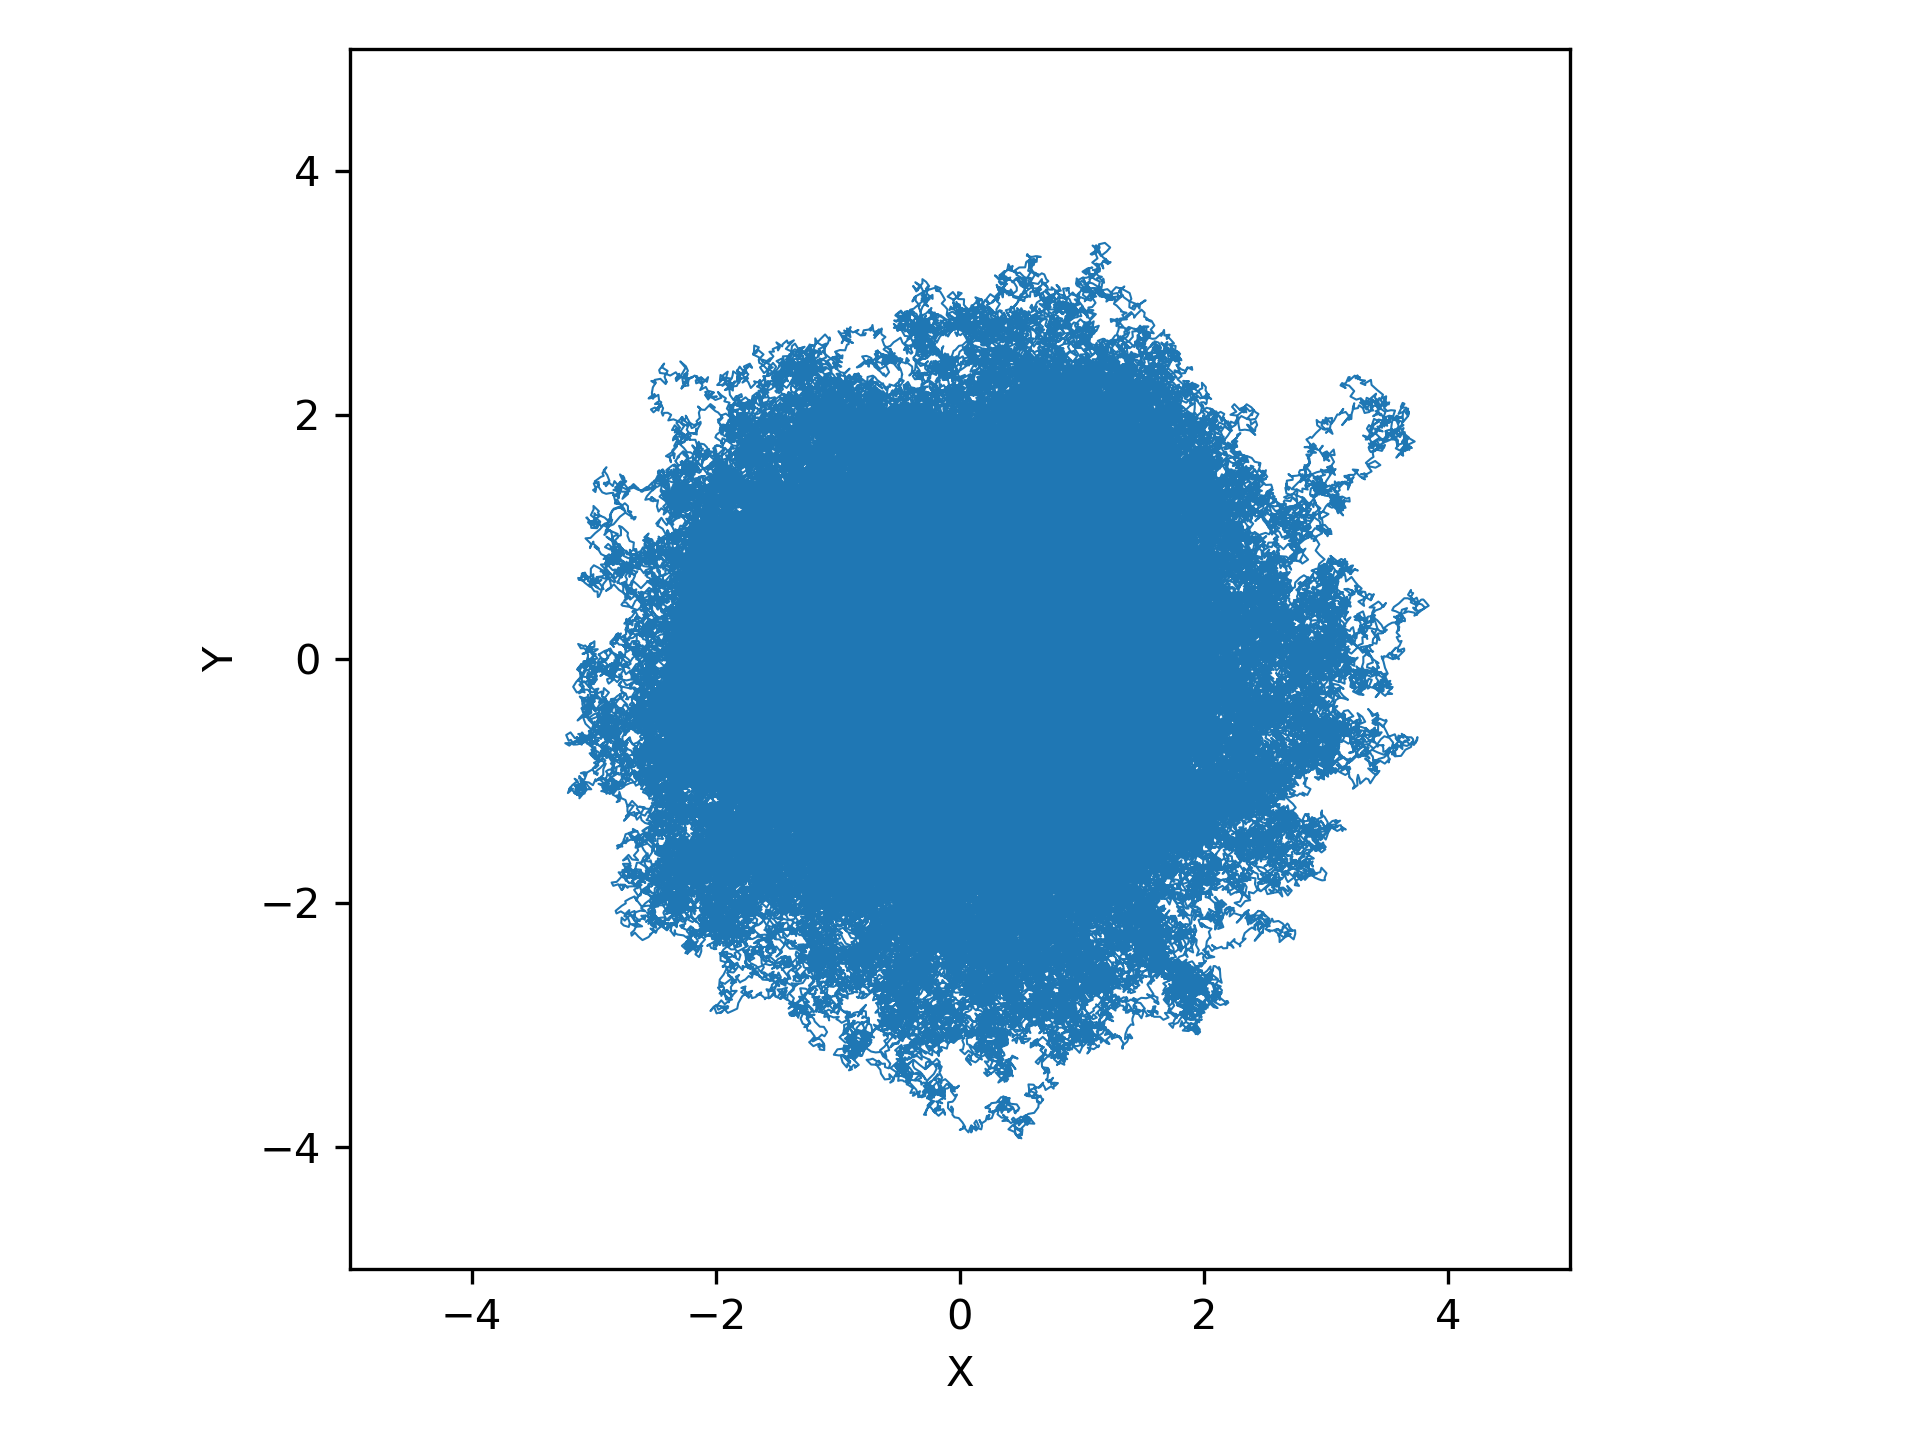
\includegraphics[bb= 0 0 460.8 345.6,width=6cm] {0.05-106-2.png}}
\subfigure[$\Delta = 0.5,n=2000$得到的Markov链]{
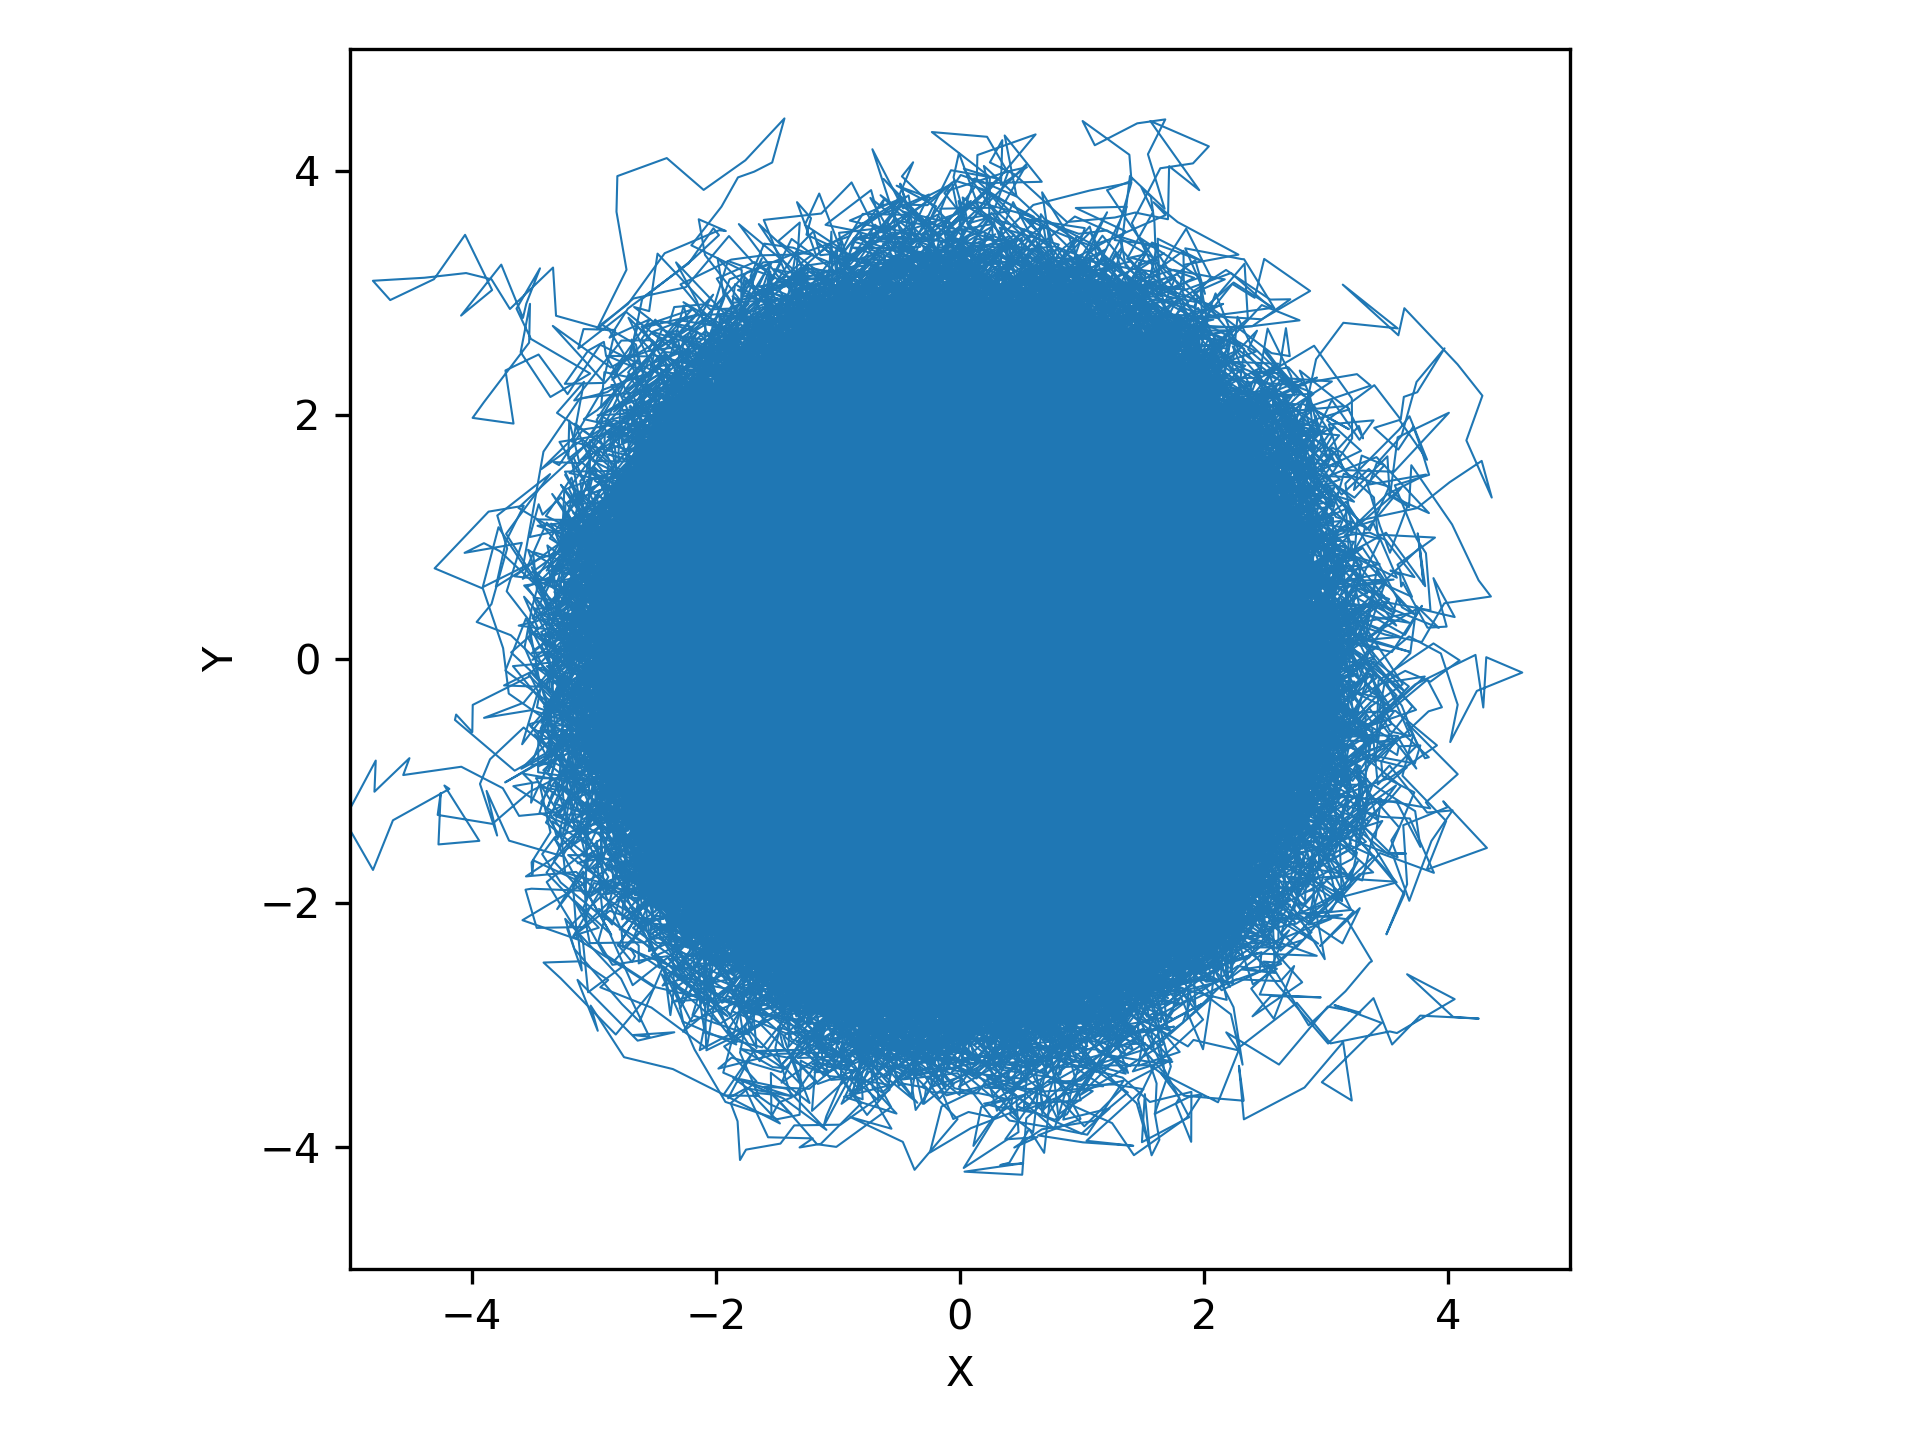
\includegraphics[bb= 0 0 460.8 345.6,width=6cm] {0.5-106-2.png}}
\subfigure[$\Delta = 5,n=1500$得到的Markov链]{
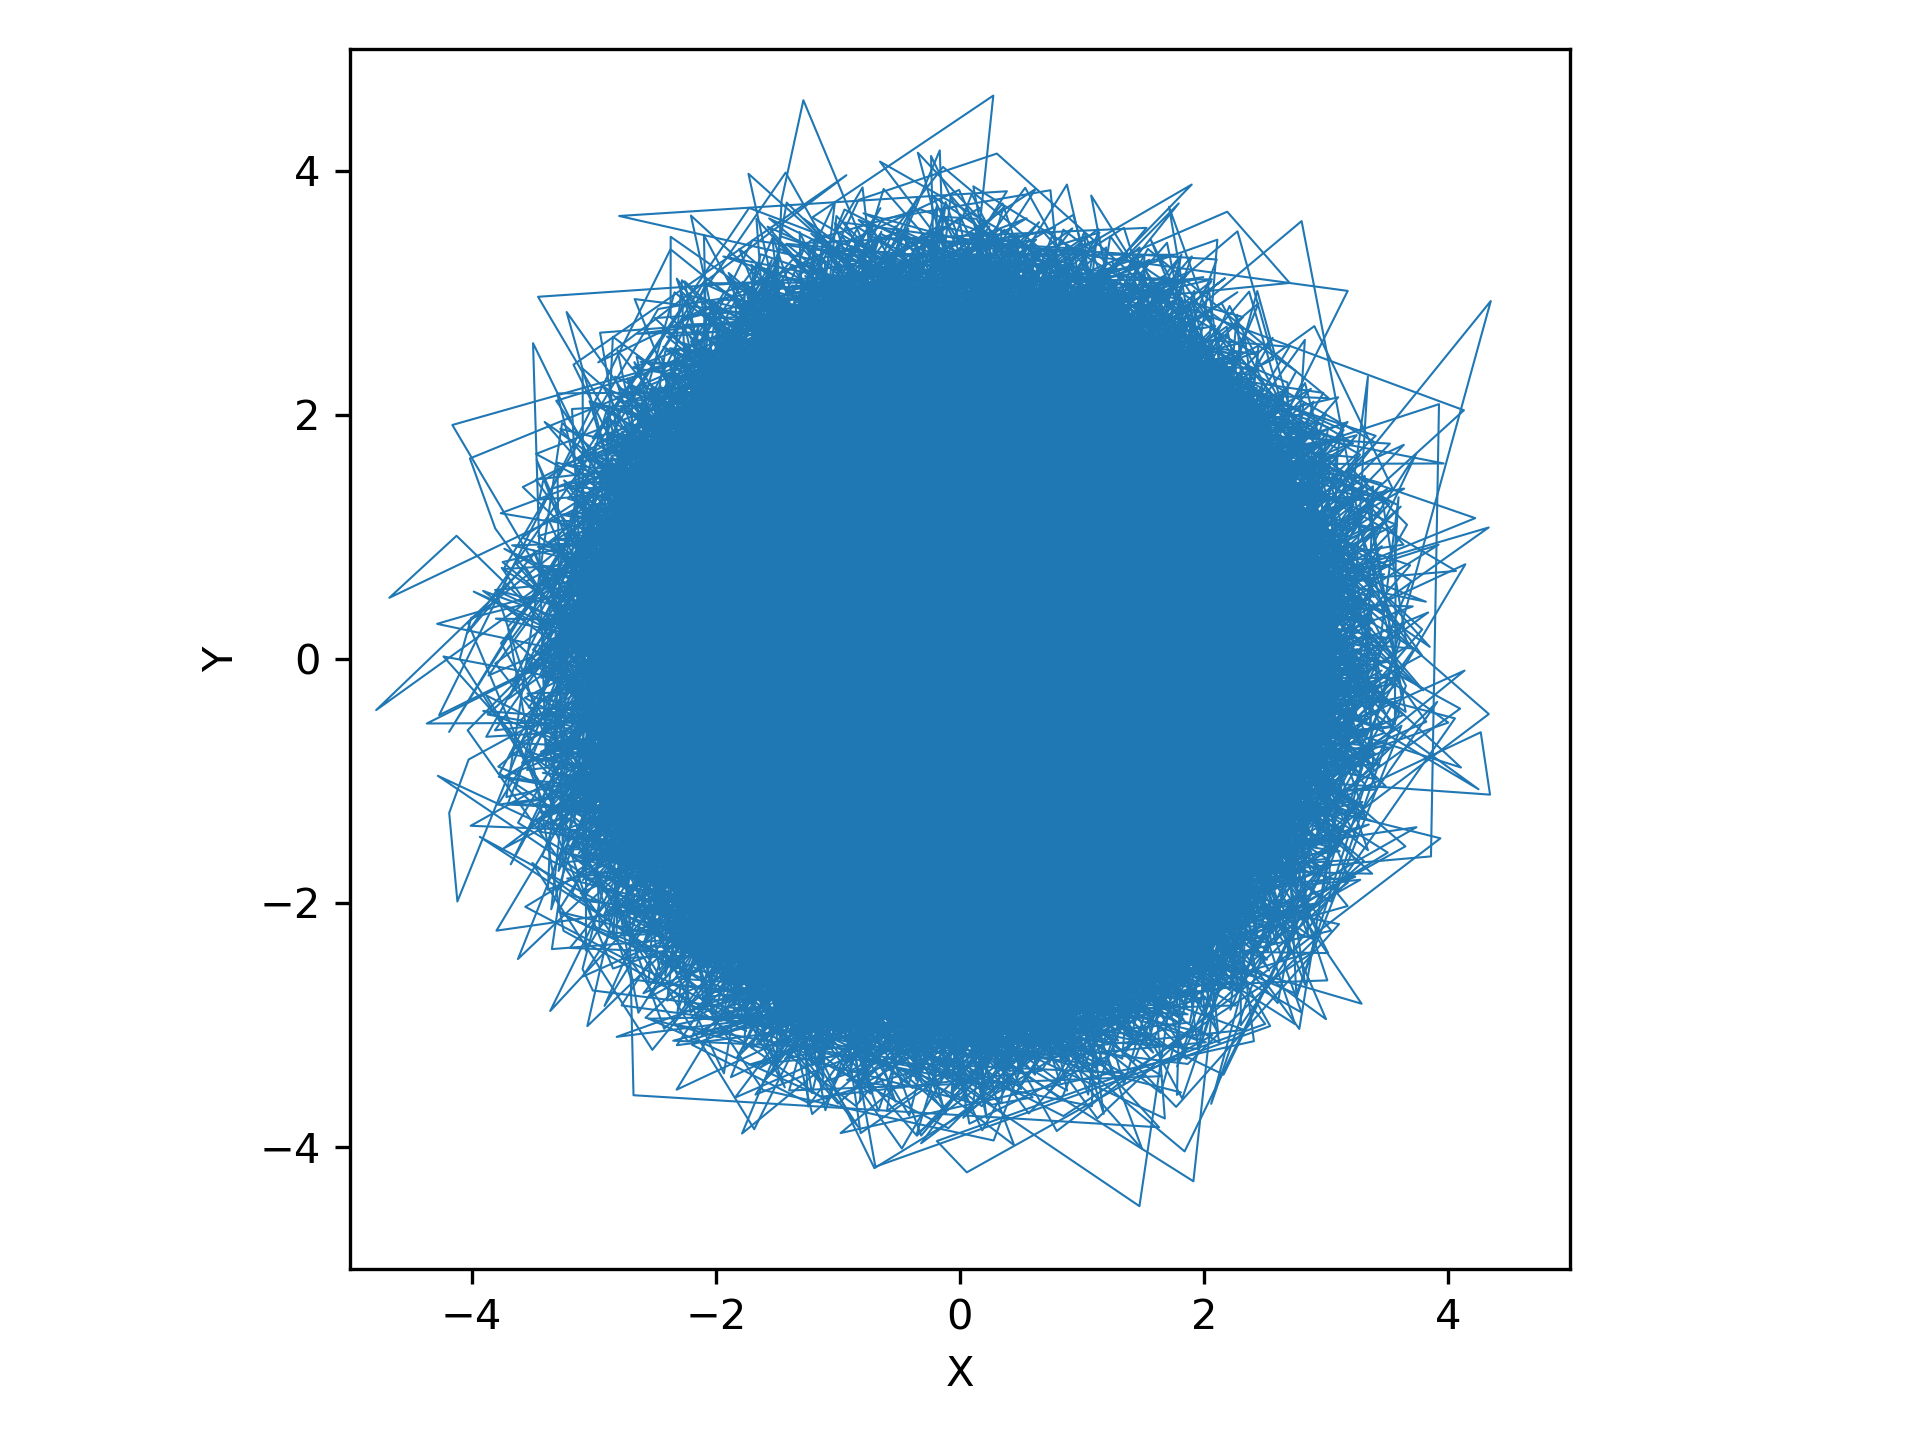
\includegraphics[bb= 0 0 460.8 345.6,width=6cm] {5-106-2.png}}
\subfigure[$\Delta = 50,n=1500$得到的Markov链]{
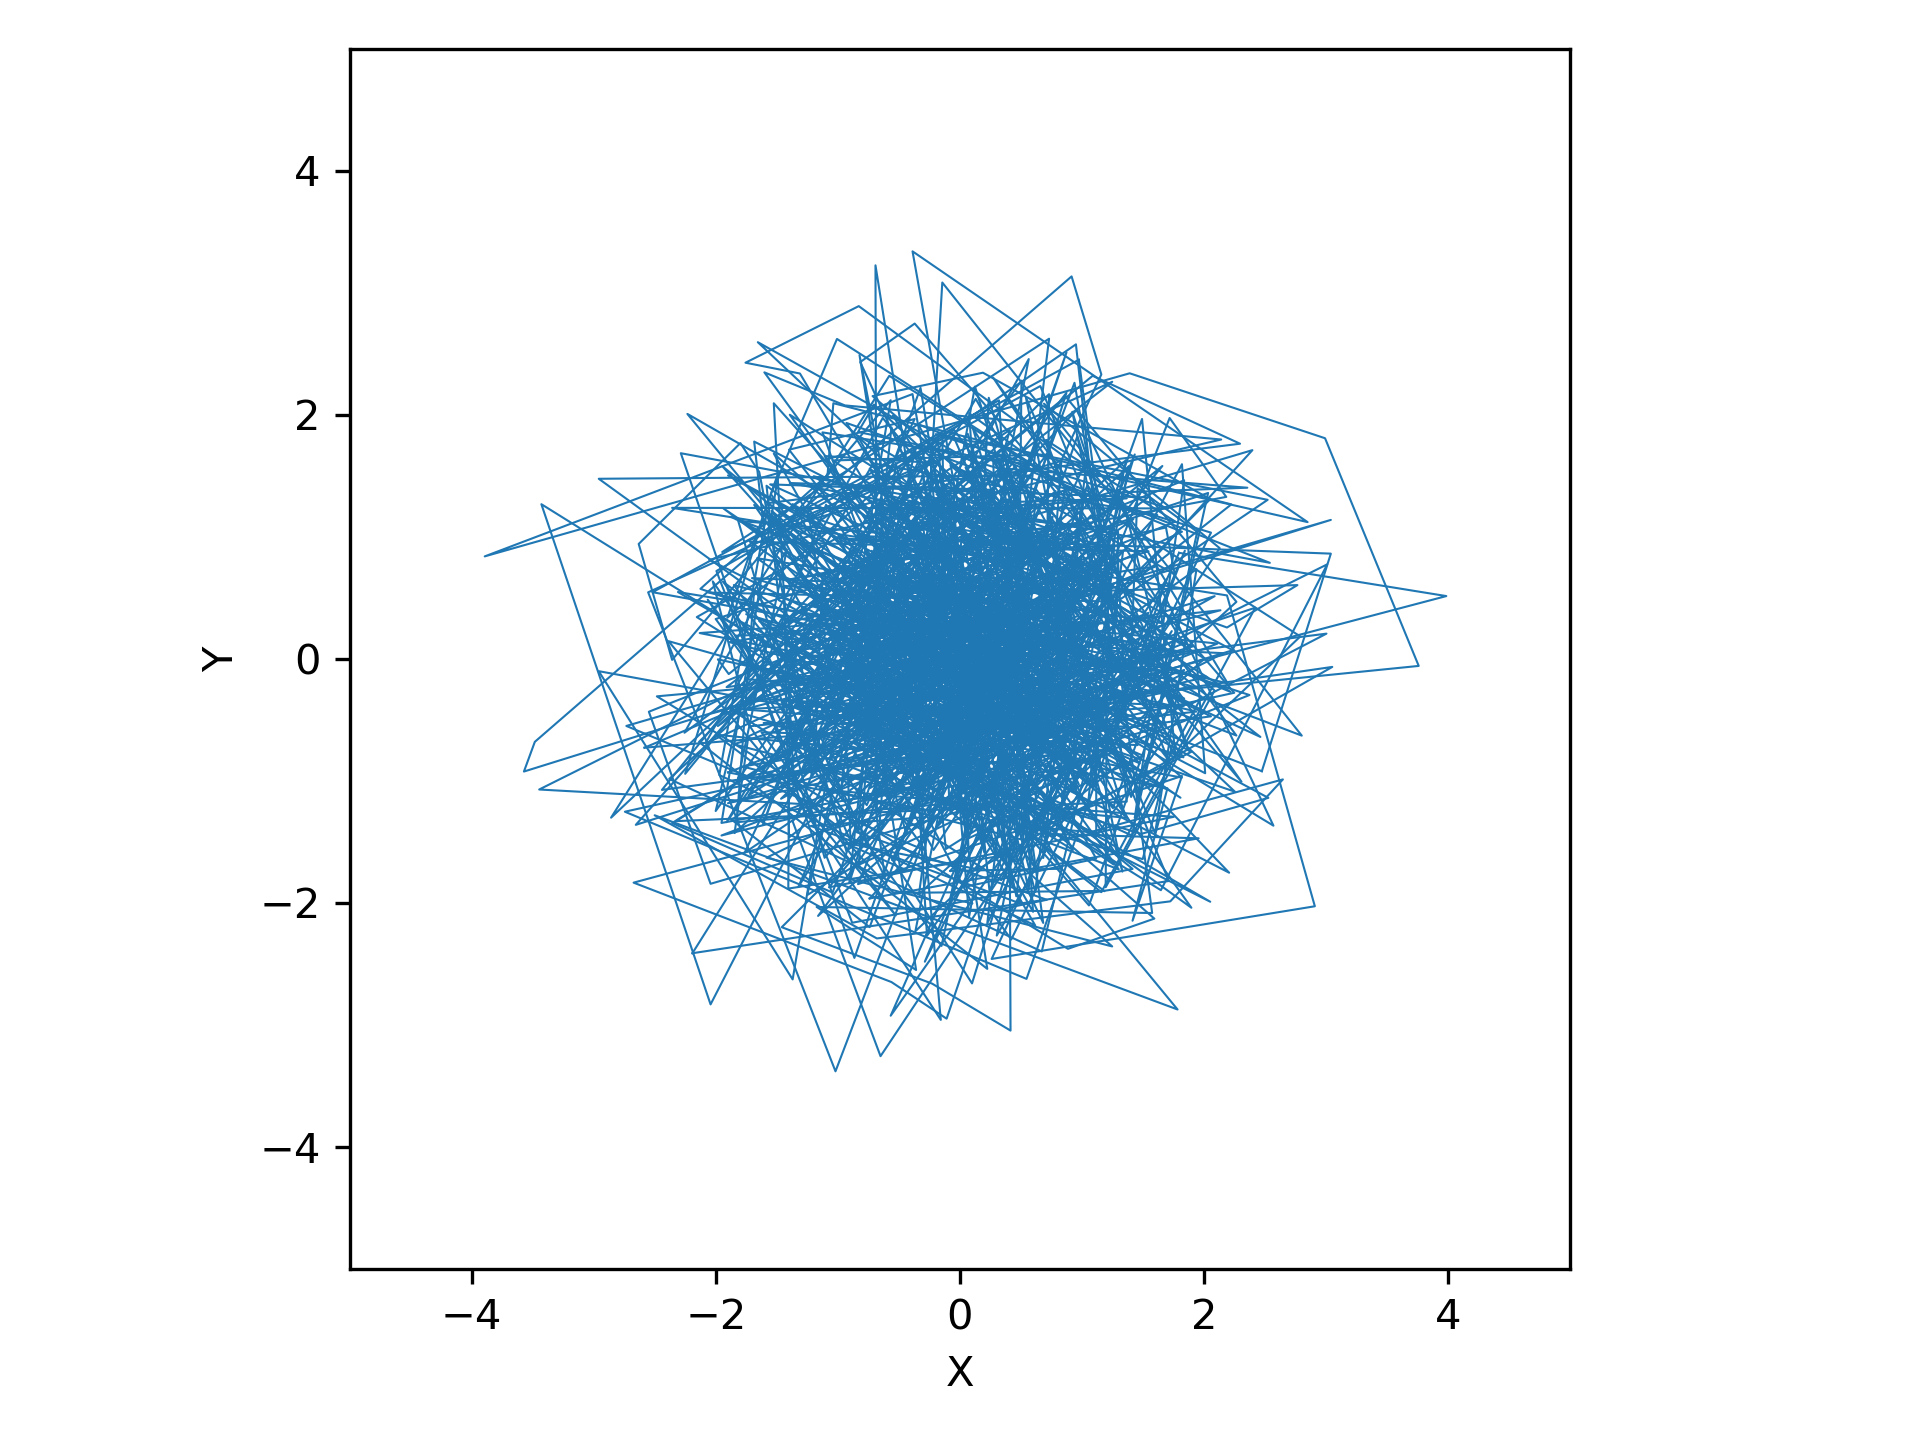
\includegraphics[bb= 0 0 460.8 345.6,width=6cm] {50-106-2.png}}
\caption{$N=10^{6}$删去前$n$个链节得到的Markov链}
\end{figure}

可以看出此时已基本消除了起始位置带来的影响。

经计算得到统计量的计算结果:

\begin{table}[!htbp]
\centering
\begin{tabular}{|c|c|c|c|c|}
\hline
$\Delta$  &$n$          &$\left < x^{2}  \right >$   &$\left < y^{2}  \right >$     &$\left < x^{2} + y^{2} \right >$     \\ \hline
$0.05$ & $5000$   &1.02657   &0.84716   &1.87372  \\ \hline
$0.1$  & $2000$   &1.06450   &0.93417   &1.99867  \\ \hline
$0.5$  & $2000$   &0.99612   &1.01576   &2.01188  \\ \hline
$1$    & $1500$   &0.99551   &0.99904   &1.99456  \\ \hline
$5$    & $1500$   &1.00770   &1.00148   &2.00918  \\ \hline
$50$   & $1500$   &0.93853   &0.93817   &1.87671  \\ \hline


\end{tabular}
\caption{共产生$10^{6}$个链节,删除前$n$个链节得到的统计量计算结果一览表}
\end{table}

从表格中可以看出,步长比较合适时,得到的统计量值才与理论值较为接近。此点也很好理解,当步长比较小的时候,每步移动的距离有限,相同步数下很难形成比较均匀的图样,需很多的步数统计量才能逼近理论值;而步长比较大时,由于移动距离比较大的情况均会不予移动到新的地方,故重复链节很多,导致统计量计算误差。

综上,利用Metropolis方法进行抽样时,步长的选择是一门学问:既不能太大,(太大得到的分布不够好)也不能太小(太小需要更多的步数才能得到好的分布),需要根据具体情况具体定下步长的取值。





\newpage
\section{附录}

\begin{appendices}


\section{Metropois算法抽样C语言源程序}
\begin{lstlisting}[language = C]
#include <stdio.h>
#include <stdlib.h>
#include <time.h>
#include <math.h>


//写文件子程序,输入写成文件名称字符串str,数据来源于数组num,数据总数n
int my_filewriter(char str[],double num[],int n){
    FILE * fp;
    fp = fopen(str,"w+");

    for(int i=0;i<(n-1);i++)
    {
        fprintf(fp,"%lf,",num[i]);

    }
    fprintf(fp,"%lf",num[n-1]);    //最后一个数据后不加 ","
    fclose(fp);
    return 0;
}



int main(int argc, const char * argv[]) {
    time_t t;
    srand((unsigned) time(&t));
    double x = 10;   //起始点的(x,y)坐标
    double y = 10;
    double sigmax = 1;   //sigmax,sigmay的值
    double sigmay = 1;
    double dE;   //能量差
    double dx,dy;  //坐标x,y某一步的该变量
    double delta = 50; //每一步的步长范围在[-delta,delat]之间
    double flag;
    int N = 1000000;   //总步数
    int n = 1500;    //计算统计量删去起始点数的个数
    double avgx2 = 0;   //计算产生数据点的<x^2>
    double avgy2 = 0;   //计算产生数据点的<y^2>
    double avgsum = 0;  //计算产生数据点的<x^2+y^2>
    
    double *positionx = malloc(sizeof(double)*N);  //存放markov链的节点坐标数组
    double *positiony = malloc(sizeof(double)*N);
    
    
    for(int i=0;i<N;){
        dx = 2*delta*rand()/(double)RAND_MAX-delta;
        dy = 2*delta*rand()/(double)RAND_MAX-delta;
           
        dE = ( pow(x+dx,2)-pow(x,2) )/(2*sigmax) + ( pow(y+dy,2)-pow(y,2) )/(2*sigmay);
        if(dE<0){
            x += dx;
            y += dy;
            positionx[i] = x;
            positiony[i] = y;
            i++;
        }
        else{
            flag = rand()/(double)RAND_MAX;
            if(flag < exp(-dE) ){
                x += dx;
                y += dy;
            }
            positionx[i] = x;
            positiony[i] = y;
            i++;
        }
    }
    
    my_filewriter("x.dat", positionx, N);
    my_filewriter("y.dat", positiony, N);
      
    if(n >= N){   //参数检查
        printf("Parameters wrong!!\n");
        return 0;
    }
    
    for(int i = n-1;i<N;i++){   //计算统计量
        avgx2 += pow(positionx[i],2)/(double)(N-n);
        avgy2 += pow(positiony[i],2)/(double)(N-n);
    }
    avgsum = avgx2 + avgy2;
    printf("average of x2 is:%.5lf\n",avgx2);
    printf("average of y2 is:%.5lf\n",avgy2);
    printf("average of x2+y2 is:%.5lf\n",avgsum);
    
   
    
    return 0;
}

\end{lstlisting}

\newpage

\section{可视化绘图及数据处理Python程序源码}
\begin{lstlisting}[language = python]
import matplotlib.pyplot as plt
import numpy as np

plt.rcParams['savefig.dpi'] = 300 #图片像素
plt.rcParams['figure.dpi'] = 300 #分辨率
# 默认的像素:[6.0,4.0],分辨率为100,图片尺寸为 600&400
fig1 = plt.figure()
fig2 = plt.figure()

ax1 = fig1.add_subplot(111)
ax2 = fig2.add_subplot(111)

X = []
Y = []
delta = 0.01  #步长
N = 6   #总链节数为10^N

with open('problem 16 Metropolis/'+str(delta)+'-10'+str(N)+'-x.dat', 'r') as f:
    while True:
        lines = f.readline() # 整行读取数据
        if not lines:
            break
        X = [float(i) for i in lines.split(',')]  # 将整行数据分割处理
    X = np.array(X) # 将数据从list类型转换为array类型。


with open('problem 16 Metropolis/'+str(delta)+'-10'+str(N)+'-y.dat', 'r') as f:
    while True:
        lines = f.readline() # 整行读取数据
        if not lines:
            break
        Y = [float(i) for i in lines.split(',')]  # 将整行数据分割处理
    Y = np.array(Y) # 将数据从list类型转换为array类型。


n = 2000

ax2.plot(np.delete(X, np.s_[0:n:1]), np.delete(Y, np.s_[0:n:1]), lw=0.5)
ax2.set_xlabel('X')
ax2.set_ylabel('Y')
ax2.set_aspect('equal')
fig2.savefig(str(delta)+'-10'+str(N)+'-2.png')
\end{lstlisting}


\end{appendices}



\end{document}
